\documentclass[a4paper, 11pt]{article}
\usepackage{uplb_gs_modified_forVPS,amssymb,amsmath,amsthm,epsfig,multicol,graphicx,url}
\usepackage{tikz}
\usepackage{amstext}
\usepackage{comment} % enables the use of multi-line comments (\ifx \fi)  
\usepackage{fullpage} % changes the margin
\usepackage{relsize} 
\usepackage{parskip} % paragraph spacing
\usepackage{url} % for reference 2
\usepackage{indentfirst}
\usepackage[margin=0.75in]{geometry}
\usepackage{commath}
\usepackage{amsmath,amsfonts,amssymb}
\newtheorem{define}{Definition}
\newtheorem{thm}{Theorem}
\newtheorem{prop}{Proposition}
\newtheorem{lem}{Lemma}
\newtheorem{cor}{Corollary}
\newtheorem{ex}{Example}
\newtheorem{pf}{Proof}
\usetikzlibrary{arrows}
\pgfarrowsdeclarecombine{twotriang}{twotriang}%
{triangle 90}{triangle 90}{triangle 90}{triangle 90}
\makeatletter
\tikzset{my loop/.style =  {to path={
			\pgfextra{\let\tikztotarget=\tikztostart}
			[looseness=5,min distance=10mm]
			\tikz@to@curve@path},font=\sffamily\small
}}  
\makeatletter 
\begin{document}
		\title{\textbf{THE GRACEFULNESS OF $F_{n}\left ( 2 \right )$ TREES}}
		\author{
		Joana Rose Dela Cruz\\
		\textit{Institute of Mathematical Sciences and Physics}\\
		\textit{University of the Philippines Los Banos}\\
		\textit{College, Laguna 4031, Philippines}	\\
		\textit{(email: jgdelacruz9@up.edu.ph)}	}
		\date{February 28, 2019}
	\maketitle
	
	\begin{center}
		\textbf{Abstract}
	\end{center}
\noindent 
\noindent Let $T$ be a tree with $n + 1$ vertices. Then, $T$ is graceful if we can label its vertices distinctly with $0,1,2,\ldots,n$ such that the induced edge labels are also distinct and run from $1$ through $n$, where the label of an edge is the absolute difference of the labels of its endvertices. \par 

For $n\geq2$, let  $F_{n}\left ( 2 \right )$ be the tree formed by considering a $J_{n}$ tree or a path $v_{0}v_{1}v_{2}\ldots v_{n-1}$ of length $n−1$ and planting to every vertex $v_{i}$ an end vertex of a path of length $i$ for
$i = 0,1,2,\ldots,n−1$. Plant an end vertex of a path $\overline{P_{2}}$ of length $2$ to every vertex $v_{1}v_{2},\ldots,v_{n}$ of $J_{n}$. We show that $J_{n}$ is graceful for each natural number n.

\section{Introduction}

\par One of the most well-known unproven conjectures in Graph Theory is the Ringel - Kotzig conjecture which is named after Gerhard Ringel and Anton Kotzig who were German and Slowak mathematicians, respectively. In 1963, Ringel and Kotzig hypothesized that all trees are graceful. That is, given a tree, we can find at least one graceful labelling. The concept of graceful labelling was initially introduced by Alexander Rosa in 1967 and the term itself was later on coined by Solomon Golomb. The Ringel - Kotzig conjecture is also known as the “graceful labeling conjecture” or the "graceful tree conjecture". \par
According to Mehendale’s proposal on Gracefully Labelling Trees, "a tree on n vertices is said to be graceful or said to have a graceful labelling if when its vertices are labelled with integers ${1, 2,\ldots, n}$ and lines (edges) are labelled by the difference of their respective end vertex labels then all the edge labels taken together constitute the set ${1, 2,\ldots, n-1}$." \par
Since the introduction of the Ringel - Kotzig conjecture, many attempts were made in order to confirm the validity of the said conjecture. However, the conjecture remains unproven until now. No direct proof has been formulated yet but it was suggested that the conjecture can be indirectly proven by assuming that there is a tree that is not graceful. With it being not graceful, it should not be isomorphic to any member of discovered families of graceful rees. This leads to the need to find and discover new families of graceful trees in order to support and further strengthen the conjecture. \par


\newpage
\section{Theoretical Background}
To give a better grasp of the problem, this chapter will introduce some basic concepts, definitions, and lemmas about graphs, trees, and gracefulness of trees which will be used throughout the paper. 

\begin{define} A \textbf{graph} $G$ is an ordered pair $(V(G),E(G))$, consisting of a non - empty set $V(G)$ of vertices and a set $E(G)$, disjoint from $V(G)$, of edges.\par	The vertices in a graph are usually represented by dots, while edges are represented by curves or segments. \par For example, if $V(G) = {v_{1},v_{2},v_{3}}$ and $E(G) = {(v_{1},v_{1}),(v_{1},v_{2}),(v_{1},v_{2}),(v_{1},v_{3}),(v_{1},v_{3}),(v_{2},v_{3})}$, then the graph may be presented as in the figure below:
	
	\begin{center}
		\resizebox {0.2\textwidth} {0.7\height} {
			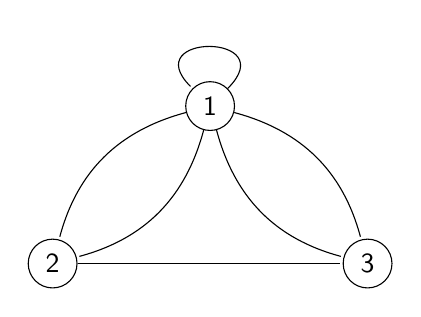
\begin{tikzpicture}[shorten >=1pt, auto, node distance=3cm,
			node_style/.style={circle,draw=black,fill=white!20!,font=\sffamily},
			edge_style/.style={draw=black}]
			\node[node_style] (n1) at (5,13)  {1};
			\node[node_style] (n2) at (3,11) {2};
			\node[node_style] (n3) at (7,11)  {3};
			\draw[edge_style]  (n2) edge node{} (n3);
			\path  (n1)   edge[my loop] node[above]  {} (n1);
			\path (n1) edge [bend left] (n2);
			\path (n1) edge [bend left] (n3);
			\path (n1) edge [bend right] (n2);
			\path (n1) edge [bend right] (n3);
			\end{tikzpicture}}
	\end{center}	
\end{define} 
\bigskip

\begin{define}  If $a\in V(G)$ and $(a,a)\in E(G)$, $(a,a)$ is called a \textbf{loop}. If $(a,b)\in E(G)$ such that $a\neq b$, $(a,b)$ is called a \textbf{link}. If $(a,b)$ occurs more than once in the edge list, it is called a \textbf{multiple edge}.
\end{define}
\bigskip

\begin{define}A graph is \textbf{simple} if it has no loops and no two of its edges join the same pair of vertices.
\end{define}
\bigskip

\begin{define} A graph is \textbf{finite} if both its vertex set and edge set are finite.
\end{define}
\bigskip

\begin{define} A \textbf{walk} in a graph $G$ is a finite nonempty sequence $W = v_{0}e_{1}v_{1}e_{2}\ldots e_{k}v_{k}$, whose terms are alternately vertices and edges of $G$, such that, for $1 ≤ i ≤ k$, the ends of $e_{i}$ are $v_{i-1}$ and $v_{i}$. A walk is \textbf{closed} if its end and initial vertices are the same. If the vertices in a walk are distinct, then the walk is called a \textbf{path}.\end{define}
\bigskip

\begin{define} A graph is \textbf{cyclic} if it has a closed path. Otherwise, it is \textbf{acyclic}.
\end{define}
\bigskip

\begin{define} A graph $G$ is \textbf{connected} if there is a path between any two vertices in $G$.
\end{define}
\bigskip

\begin{define} A \textbf{tree} is an acyclic connected simple graph.	
\end{define} \bigskip

\begin{define} A \textbf{graceful numbering} or \textbf{valuation} of a graph $G$ with $m$ edges is	an injection $g$ between the vertex set $V (G)$ of $G$ and $N^0_{m} = {0,1,\ldots,m}$ such that the induced function $w$ defined as $w(u,v) = |g(u)−g(v)|$ is a bijection between the edge set $E(G)$ and $N_{m} = {1,2,\ldots,m}$.
\end{define}
\bigskip

\begin{define} A graph with a graceful numbering is called a \textbf{graceful graph}
\end{define}
\bigskip

\newpage
\section{Review of Related Literature}

Over the course of more than five decades, attempts on proving the Graceful
Tree Conjecture only resulted to the discovery of new classes or families of graceful trees. Even though an algorithm that can generate all graceful trees has not been developed yet, studies regarding the conjecture can contribute to strengthening it as more families of graceful trees are discovered. Here are several classes of trees cited by Gallian in his book “A Dynamic Survey of Graph Labeling” known to be graceful.
\bigskip
\begin{enumerate}
	
	\item \noindent {\bfseries Path}\\
	A path (or chain) is a walk with distinct vertices and edges. Shown in the figure below is a gracefully-labeled path on 7 vertices.\\
	
	\begin{center}
		\resizebox {0.5\textwidth} {0.5\height} {
			
			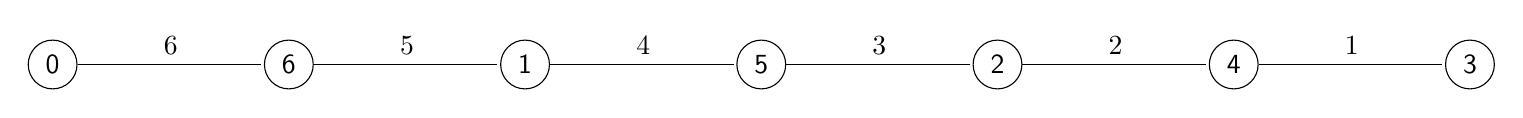
\begin{tikzpicture}[shorten >=1pt, auto, node distance=3cm,
			node_style/.style={circle,draw=black,fill=white!20!,font=\sffamily},
			edge_style/.style={draw=black}]
			\node[node_style] (n0) at (4,9)  {0};
			\node[node_style] (n6) at (7,9) {6};
			\node[node_style] (n1) at (10,9)  {1};
			\node[node_style] (n5) at (13,9)  {5};
			\node[node_style] (n2) at (16,9) {2};
			\node[node_style] (n4) at (19,9)  {4};
			\node[node_style] (n3) at (22,9)  {3};
			\draw[edge_style]  (n0) edge node{6} (n6);
			\draw[edge_style]  (n6) edge node{5} (n1);
			\draw[edge_style]  (n1) edge node{4} (n5);
			\draw[edge_style]  (n5) edge node{3} (n2);
			\draw[edge_style]  (n2) edge node{2} (n4);
			\draw[edge_style]  (n4) edge node{1} (n3);
			\end{tikzpicture}}
	\end{center}
	
	
	
	\bigskip
	\item \noindent {\bfseries Caterpillars}\\
	A caterpillar is a tree where the removal of its vertices of degree one leaves a path. Shown in the figure below is a gracefully-labeled caterpillar on 14 vertices.\\
	\begin{center}
		\resizebox {0.6\textwidth} {0.5\height} {
			\begin{tikzpicture}[shorten >=1pt, auto, node distance=3cm,
			node_style/.style={circle,draw=black,fill=white!20!,font=\sffamily},
			edge_style/.style={draw=black}]
			\node[node_style] (n12) at (7,11)  {12};
			\node[node_style] (n9) at (13,11) {9};
			\node[node_style] (n5) at (16,11)  {5};
			\node[node_style] (n13) at (3,9)  {13};
			\node[node_style] (n2) at (7,9) {2};
			\node[node_style] (n10) at (10,9)  {10};
			\node[node_style] (n4) at (13,9)  {4};
			\node[node_style] (n8) at (16,9)  {8};
			\node[node_style] (n6) at (19,9) {6};
			\node[node_style] (n0) at (1,7)  {0};
			\node[node_style] (n1) at (4,7)  {1};
			\node[node_style] (n11) at (7,7) {11};
			\node[node_style] (n3) at (10,7)  {3};
			\node[node_style] (n7) at (16,7)  {7};
			\draw[edge_style]  (n0) edge node{13} (n13);
			\draw[edge_style]  (n1) edge node{12} (n13);
			\draw[edge_style]  (n2) edge node{11} (n13);
			\draw[edge_style]  (n2) edge node{9} (n11);
			\draw[edge_style]  (n2) edge node{10} (n12);
			\draw[edge_style]  (n2) edge node{8} (n10);
			\draw[edge_style]  (n3) edge node{7} (n10);
			\draw[edge_style]  (n4) edge node{6} (n10);
			\draw[edge_style]  (n4) edge node{5} (n9);
			\draw[edge_style]  (n4) edge node{4} (n8);
			\draw[edge_style]  (n5) edge node{3} (n8);
			\draw[edge_style]  (n7) edge node{1} (n8);
			\draw[edge_style]  (n8) edge node{2} (n6);
			\end{tikzpicture}}
	\end{center}	
	\bigskip
	\item \noindent {\bfseries Symmetrical Trees}\\
	A symmetrical tree is a rooted tree in which every level contains vertices of the same degree. Shown in the figure below is a gracefully-labeled symmetrical tree on 11 vertices.\\
	\begin{center}
		\resizebox {0.3\textwidth} {0.5\height} {
			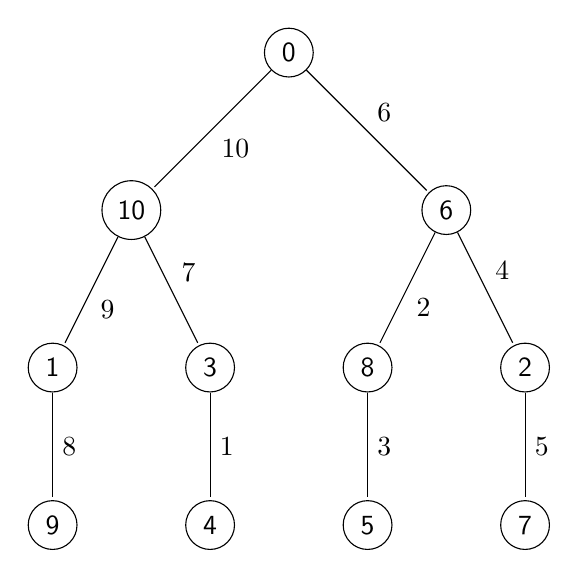
\begin{tikzpicture}[shorten >=1pt, auto, node distance=3cm,
			node_style/.style={circle,draw=black,fill=white!20!,font=\sffamily},
			edge_style/.style={draw=black}]
			\node[node_style] (n0) at (5,13)  {0};
			\node[node_style] (n10) at (3,11) {10};
			\node[node_style] (n6) at (7,11)  {6};
			\node[node_style] (n1) at (2,9) {1};
			\node[node_style] (n3) at (4,9)  {3};
			\node[node_style] (n8) at (6,9)  {8};
			\node[node_style] (n2) at (8,9)  {2};
			\node[node_style] (n9) at (2,7) {9};
			\node[node_style] (n4) at (4,7)  {4};
			\node[node_style] (n5) at (6,7)  {5};
			\node[node_style] (n7) at (8,7)  {7};
			\draw[edge_style]  (n0) edge node{10} (n10);
			\draw[edge_style]  (n0) edge node{6} (n6);
			\draw[edge_style]  (n10) edge node{9} (n1);
			\draw[edge_style]  (n10) edge node{7} (n3);
			\draw[edge_style]  (n6) edge node{2} (n8);
			\draw[edge_style]  (n6) edge node{4} (n2);
			\draw[edge_style]  (n1) edge node{8} (n9);
			\draw[edge_style]  (n3) edge node{1} (n4);
			\draw[edge_style]  (n8) edge node{3} (n5);
			\draw[edge_style]  (n2) edge node{5} (n7);
			\end{tikzpicture}}
	\end{center}	
	\bigskip
	\item \noindent {\bfseries Spider Trees}\\
	A spider tree is a tree with one vertex of degree at least 3 and all others with degree at most 2. Shown in the figure below is a gracefully-labeled spider tree on 7 vertices.\\
	\begin{center}
		\resizebox {0.2\textwidth} {0.4\height} {
			\begin{tikzpicture}[shorten >=1pt, auto, node distance=3cm,
			node_style/.style={circle,draw=black,fill=white!20!,font=\sffamily},
			edge_style/.style={draw=black}]
			\node[node_style] (n5) at (1,13)  {5};
			\node[node_style] (n1) at (9,13) {1};
			\node[node_style] (n0) at (3,11)  {0};
			\node[node_style] (n4) at (7,11) {4};
			\node[node_style] (n6) at (5,9)  {6};
			\node[node_style] (n2) at (5,7)  {2};
			\node[node_style] (n3) at (5,5)  {3};
			\draw[edge_style]  (n5) edge node{5} (n0);
			\draw[edge_style]  (n1) edge node{3} (n4);
			\draw[edge_style]  (n0) edge node{6} (n6);
			\draw[edge_style]  (n4) edge node{2} (n6);
			\draw[edge_style]  (n6) edge node{4} (n2);
			\draw[edge_style]  (n3) edge node{1} (n2);
			\end{tikzpicture}}
	\end{center}	
	\bigskip
	\item \noindent {\bfseries Stars}\\
	A star is a special case of caterpillar where the deletion of its end vertices results into a single vertex or a point. Shown in the figure below is a gracefully-labeled star of 5 vertices.\\
	\begin{center}
		\resizebox {0.15\textwidth} {0.4\height} {
			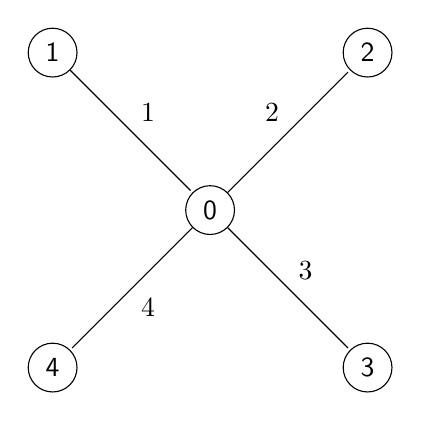
\begin{tikzpicture}[shorten >=1pt, auto, node distance=3cm,
			node_style/.style={circle,draw=black,fill=white!20!,font=\sffamily},
			edge_style/.style={draw=black}]
			\node[node_style] (n1) at (3,11)  {1};
			\node[node_style] (n4) at (3,7) {4};
			\node[node_style] (n0) at (5,9)  {0};
			\node[node_style] (n2) at (7,11) {2};
			\node[node_style] (n3) at (7,7)  {3};
			\draw[edge_style]  (n1) edge node{1} (n0);
			\draw[edge_style]  (n0) edge node{4} (n4);
			\draw[edge_style]  (n0) edge node{2} (n2);
			\draw[edge_style]  (n0) edge node{3} (n3);
			\end{tikzpicture}}
	\end{center}	
	
	\bigskip
	\item \noindent {\bfseries $M$-stars}\\
	A tree with one vertex acting as the root of paths of length $m$ is called an $m$-star. Shown in the figure below is a gracefully-labeled 3-star of 13 vertices.\\
	\begin{center}
		\resizebox {0.2\textwidth} {0.4\height} {
			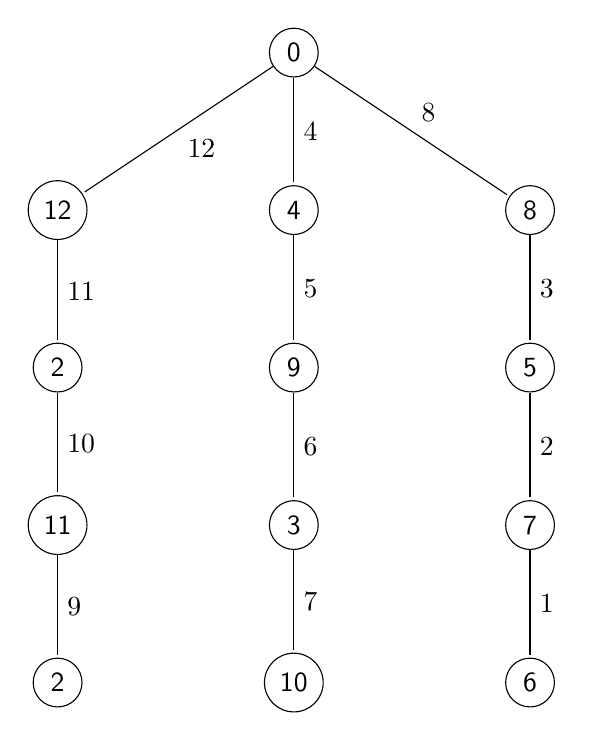
\begin{tikzpicture}[shorten >=1pt, auto, node distance=3cm,
			node_style/.style={circle,draw=black,fill=white!20!,font=\sffamily},
			edge_style/.style={draw=black}]
			\node[node_style] (n0) at (4,13)  {0};
			\node[node_style] (n12) at (1,11) {12};
			\node[node_style] (n4) at (4,11)  {4};
			\node[node_style] (n8) at (7,11) {8};
			\node[node_style] (n1) at (1,9)  {2};
			\node[node_style] (n9) at (4,9)  {9};
			\node[node_style] (n5) at (7,9)  {5};	
			\node[node_style] (n11) at (1,7) {11};
			\node[node_style] (n3) at (4,7)  {3};
			\node[node_style] (n7) at (7,7) {7};
			\node[node_style] (n2) at (1,5)  {2};
			\node[node_style] (n10) at (4,5)  {10};
			\node[node_style] (n6) at (7,5)  {6};
			\draw[edge_style]  (n0) edge node{12} (n12);
			\draw[edge_style]  (n0) edge node{4} (n4);
			\draw[edge_style]  (n0) edge node{8} (n8);
			\draw[edge_style]  (n12) edge node{11} (n1);
			\draw[edge_style]  (n1) edge node{10} (n11);
			\draw[edge_style]  (n11) edge node{9} (n2);
			\draw[edge_style]  (n4) edge node{5} (n9);
			\draw[edge_style]  (n9) edge node{6} (n3);
			\draw[edge_style]  (n3) edge node{7} (n10);
			\draw[edge_style]  (n8) edge node{3} (n5);
			\draw[edge_style]  (n5) edge node{2} (n7);
			\draw[edge_style]  (n7) edge node{1} (n6);
			\end{tikzpicture}}
	\end{center}	
	\bigskip
	\item \noindent {\bfseries Banana Trees}\\
	A banana tree is a graph obtained by joining an end vertex of a star to a single vertex not in the star by an edge. Shown in the figure below is a gracefully-labeled banana tree of 11 vertices.\\
	\begin{center}
		\resizebox {0.3\textwidth} {0.5\height} {
			\begin{tikzpicture}[shorten >=1pt, auto, node distance=3cm,
			node_style/.style={circle,draw=black,fill=white!20!,font=\sffamily},
			edge_style/.style={draw=black}]
			\node[node_style] (n1) at (6,11)  {1};
			\node[node_style] (n8) at (3,9) {8};
			\node[node_style] (n7) at (6,9)  {7};
			\node[node_style] (n5) at (9,9) {5};
			\node[node_style] (n0) at (3,7)  {0};
			\node[node_style] (n2) at (6,7)  {2};
			\node[node_style] (n6) at (9,7)  {6};	
			\node[node_style] (n9) at (1,5) {9};
			\node[node_style] (n10) at (5,5)  {10};
			\node[node_style] (n3) at (7,5) {3};
			\node[node_style] (n4) at (11,5)  {4};
			\draw[edge_style]  (n1) edge node{7} (n8);
			\draw[edge_style]  (n1) edge node{6} (n7);
			\draw[edge_style]  (n1) edge node{4} (n5);
			\draw[edge_style]  (n8) edge node{8} (n0);
			\draw[edge_style]  (n7) edge node{5} (n2);
			\draw[edge_style]  (n5) edge node{1} (n6);
			\draw[edge_style]  (n0) edge node{9} (n9);
			\draw[edge_style]  (n0) edge node{10} (n10);
			\draw[edge_style]  (n6) edge node{3} (n3);
			\draw[edge_style]  (n6) edge node{2} (n4);
			
			\end{tikzpicture}}
	\end{center}		
	\bigskip
	\item \noindent {\bfseries Firecrackers}\\
	A firecracker is a tree consisting of a path $P$ and a collection of stars, where each vertex of $P$ is joined to the central vertex of exactly one star. Shown in the figure below is a gracefully-labeled firecracker of 9 vertices.\\
	\begin{center}
		\resizebox {0.3\textwidth} {0.5\height} {
			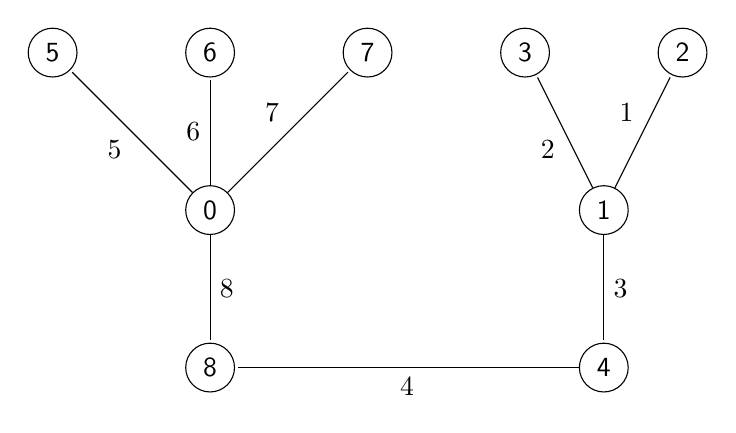
\begin{tikzpicture}[shorten >=1pt, auto, node distance=3cm,
			node_style/.style={circle,draw=black,fill=white!20!,font=\sffamily},
			edge_style/.style={draw=black}]
			\node[node_style] (n5) at (1,11)  {5};
			\node[node_style] (n6) at (3,11) {6};
			\node[node_style] (n7) at (5,11)  {7};
			\node[node_style] (n3) at (7,11) {3};
			\node[node_style] (n2) at (9,11)  {2};
			\node[node_style] (n0) at (3,9)  {0};
			\node[node_style] (n1) at (8,9)  {1};	
			\node[node_style] (n8) at (3,7) {8};
			\node[node_style] (n4) at (8,7)  {4};
			\draw[edge_style]  (n0) edge node{5} (n5);
			\draw[edge_style]  (n0) edge node{6} (n6);
			\draw[edge_style]  (n0) edge node{7} (n7);
			\draw[edge_style]  (n0) edge node{8} (n8);
			\draw[edge_style]  (n1) edge node{1} (n2);
			\draw[edge_style]  (n1) edge node{2} (n3);
			\draw[edge_style]  (n1) edge node{3} (n4);
			\draw[edge_style]  (n4) edge node{4} (n8);		
			\end{tikzpicture}}
	\end{center}		
	
	\bigskip
	\item \noindent {\bfseries Lobster Trees}\\
	A lobster tree is a tree such that the removal of its leaves results into a caterpillar. Shown in the figure below is a gracefully-labeled lobster tree of 26 vertices.\\
	\begin{center}
		\resizebox {0.9\textwidth} {0.4\height} {
			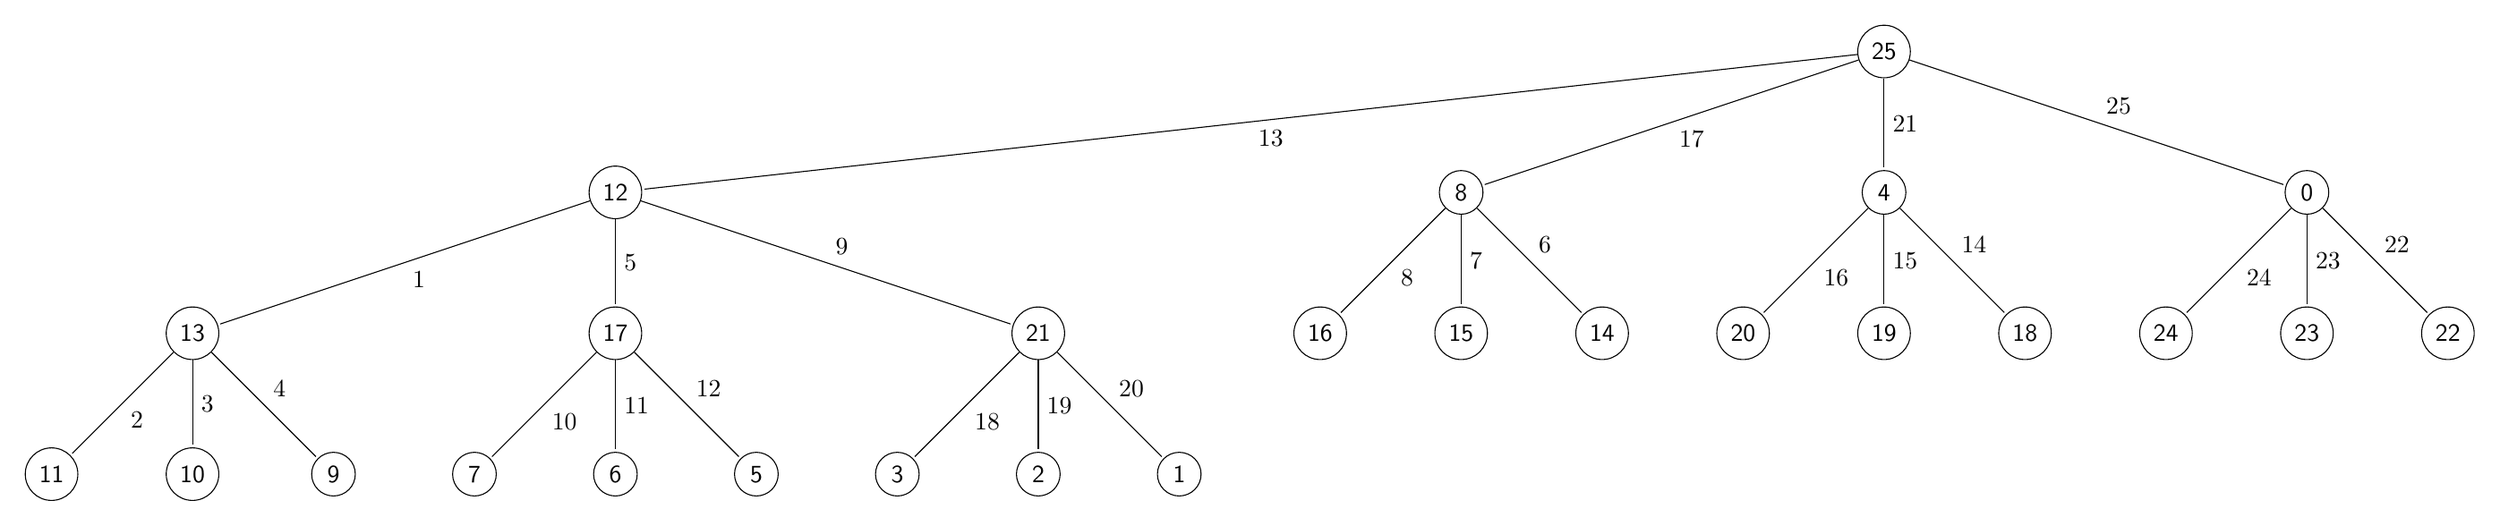
\begin{tikzpicture}[shorten >=1pt, auto, node distance=3cm,
			node_style/.style={circle,draw=black,fill=white!20!,font=\sffamily},
			edge_style/.style={draw=black}]
			\node[node_style] (n25) at (27,13)  {25};
			\node[node_style] (n12) at (9,11) {12};
			\node[node_style] (n8) at (21,11)  {8};
			\node[node_style] (n4) at (27,11) {4};
			\node[node_style] (n0) at (33,11)  {0};
			\node[node_style] (n13) at (3,9)  {13};
			\node[node_style] (n17) at (9,9)  {17};	
			\node[node_style] (n21) at (15,9) {21};
			\node[node_style] (n16) at (19,9)  {16};
			\node[node_style] (n15) at (21,9)  {15};
			\node[node_style] (n14) at (23,9) {14};
			\node[node_style] (n20) at (25,9)  {20};
			\node[node_style] (n19) at (27,9) {19};
			\node[node_style] (n18) at (29,9)  {18};
			\node[node_style] (n24) at (31,9)  {24};
			\node[node_style] (n23) at (33,9)  {23};	
			\node[node_style] (n22) at (35,9) {22};
			\node[node_style] (n11) at (1,7)  {11};
			\node[node_style] (n10) at (3,7) {10};
			\node[node_style] (n9) at (5,7)  {9};
			\node[node_style] (n7) at (7,7) {7};
			\node[node_style] (n6) at (9,7)  {6};
			\node[node_style] (n5) at (11,7)  {5};
			\node[node_style] (n3) at (13,7)  {3};	
			\node[node_style] (n2) at (15,7) {2};
			\node[node_style] (n1) at (17,7)  {1};
			\draw[edge_style]  (n25) edge node{13} (n12);
			\draw[edge_style]  (n25) edge node{17} (n8);
			\draw[edge_style]  (n25) edge node{21} (n4);
			\draw[edge_style]  (n25) edge node{25} (n0);
			\draw[edge_style]  (n12) edge node{1} (n13);
			\draw[edge_style]  (n12) edge node{5} (n17);
			\draw[edge_style]  (n12) edge node{9} (n21);
			\draw[edge_style]  (n8) edge node{8} (n16);
			\draw[edge_style]  (n8) edge node{7} (n15);
			\draw[edge_style]  (n8) edge node{6} (n14);
			\draw[edge_style]  (n4) edge node{16} (n20);
			\draw[edge_style]  (n4) edge node{15} (n19);
			\draw[edge_style]  (n4) edge node{14} (n18);
			\draw[edge_style]  (n0) edge node{24} (n24);
			\draw[edge_style]  (n0) edge node{23} (n23);
			\draw[edge_style]  (n0) edge node{22} (n22);
			\draw[edge_style]  (n13) edge node{2} (n11);
			\draw[edge_style]  (n13) edge node{3} (n10);
			\draw[edge_style]  (n13) edge node{4} (n9);
			\draw[edge_style]  (n17) edge node{10} (n7);
			\draw[edge_style]  (n17) edge node{11} (n6);
			\draw[edge_style]  (n17) edge node{12} (n5);
			\draw[edge_style]  (n21) edge node{18} (n3);
			\draw[edge_style]  (n21) edge node{19} (n2);
			\draw[edge_style]  (n21) edge node{20} (n1);
			\end{tikzpicture}}
	\end{center}		
	
	\bigskip
	\item \noindent {\bfseries Regular Bamboo Trees}\\
	A regular bamboo tree consists of legs with equal lengths attached to a
	single vertex. The leaves of this tree are leaves of stars with the same size. Shown in the figure below is a gracefully-labeled regular bamboo tree of 43 vertices.\\
	\begin{center}
		\resizebox {0.9\textwidth} {0.4\height} {
			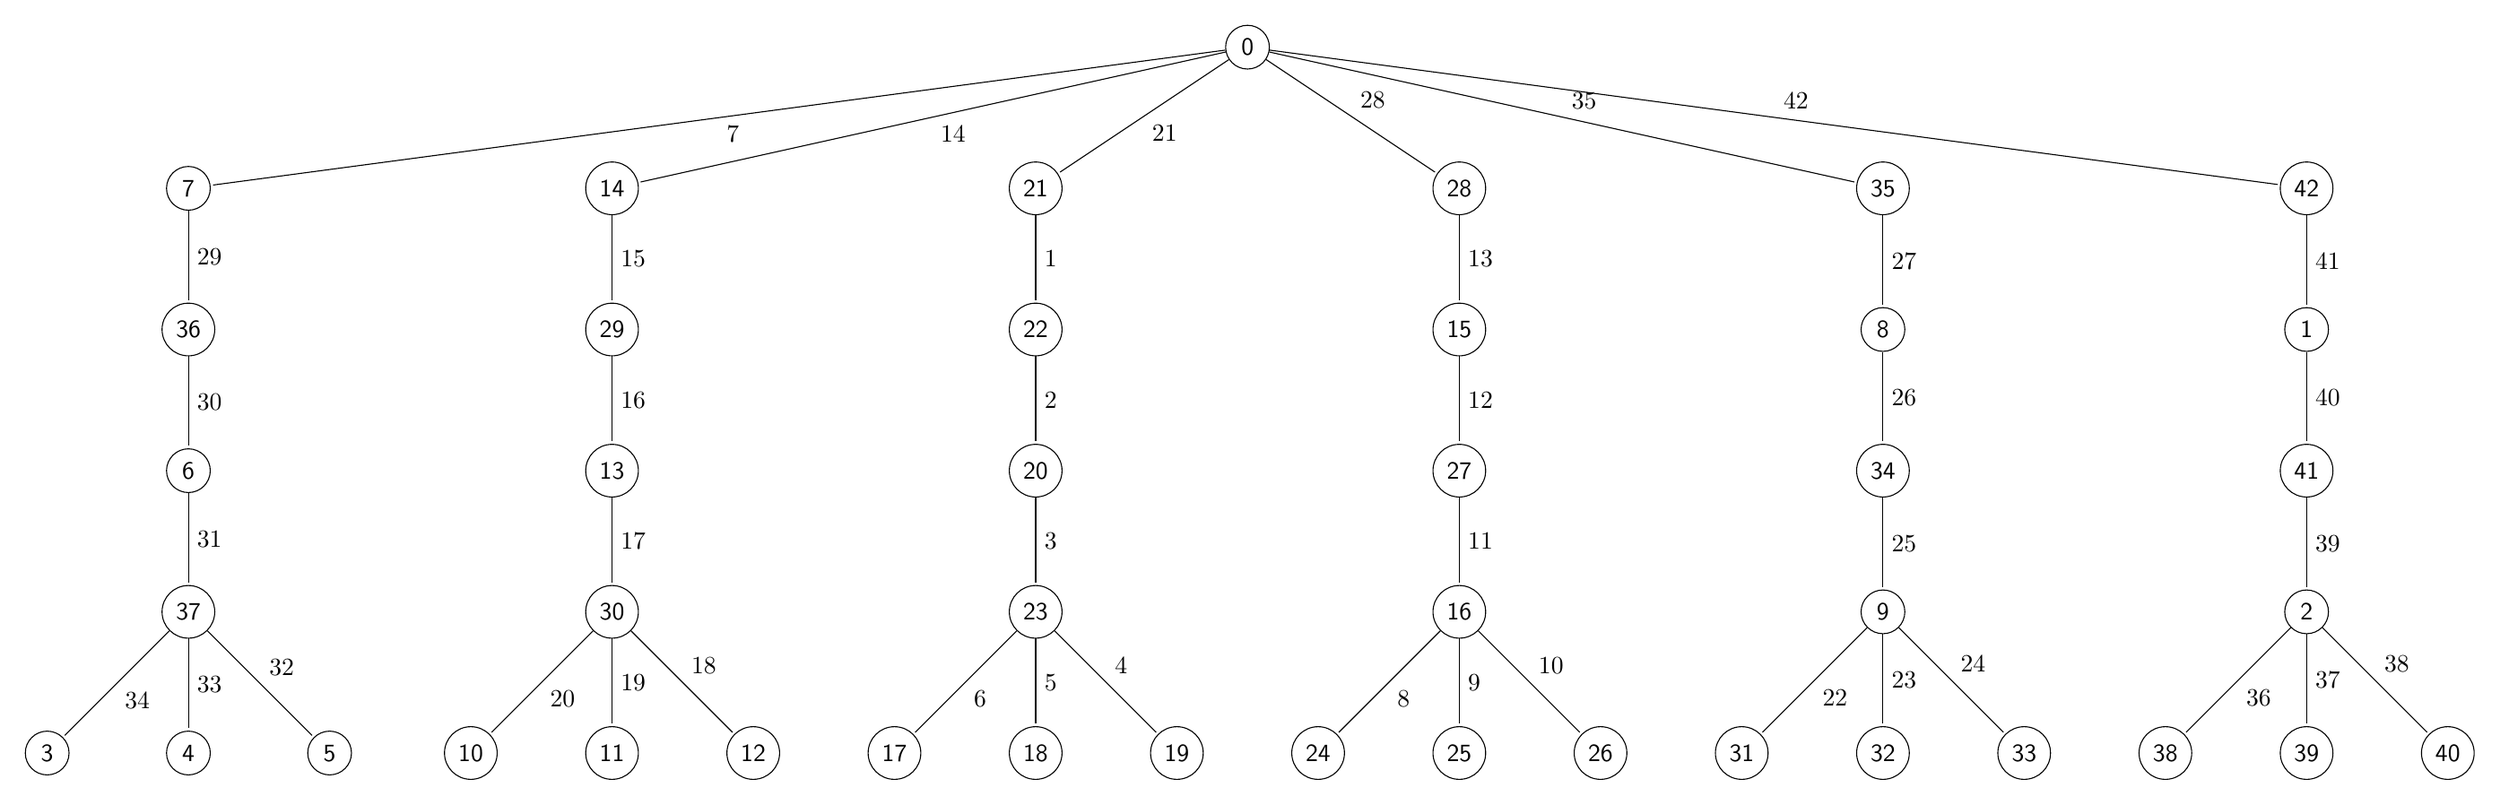
\begin{tikzpicture}[shorten >=1pt, auto, node distance=3cm,
			node_style/.style={circle,draw=black,fill=white!20!,font=\sffamily},
			edge_style/.style={draw=black}]
			\node[node_style] (n0) at (18,13)  {0};
			\node[node_style] (n42) at (33,11) {42};
			\node[node_style] (n35) at (27,11)  {35};
			\node[node_style] (n28) at (21,11) {28};
			\node[node_style] (n21) at (15,11)  {21};
			\node[node_style] (n14) at (9,11)  {14};
			\node[node_style] (n7) at (3,11)  {7};	
			\node[node_style] (n1) at (33,9) {1};
			\node[node_style] (n8) at (27,9)  {8};
			\node[node_style] (n15) at (21,9)  {15};
			\node[node_style] (n22) at (15,9)  {22};
			\node[node_style] (n29) at (9,9) {29};
			\node[node_style] (n36) at (3,9)  {36};
			\node[node_style] (n41) at (33,7)  {41};
			\node[node_style] (n34) at (27,7)  {34};	
			\node[node_style] (n27) at (21,7) {27};
			\node[node_style] (n20) at (15,7)  {20};
			\node[node_style] (n13) at (9,7) {13};
			\node[node_style] (n6) at (3,7)  {6};
			\node[node_style] (n2) at (33,5) {2};
			\node[node_style] (n9) at (27,5)  {9};
			\node[node_style] (n16) at (21,5)  {16};
			\node[node_style] (n23) at (15,5)  {23};	
			\node[node_style] (n30) at (9,5) {30};
			\node[node_style] (n37) at (3,5)  {37};
			\node[node_style] (n40) at (35,3)  {40};
			\node[node_style] (n39) at (33,3) {39};
			\node[node_style] (n38) at (31,3)  {38};
			\node[node_style] (n33) at (29,3) {33};
			\node[node_style] (n32) at (27,3)  {32};
			\node[node_style] (n31) at (25,3)  {31};
			\node[node_style] (n26) at (23,3)  {26};	
			\node[node_style] (n25) at (21,3) {25};
			\node[node_style] (n24) at (19,3)  {24};
			\node[node_style] (n19) at (17,3) {19};
			\node[node_style] (n18) at (15,3)  {18};
			\node[node_style] (n17) at (13,3) {17};
			\node[node_style] (n12) at (11,3)  {12};
			\node[node_style] (n11) at (9,3)  {11};
			\node[node_style] (n10) at (7,3)  {10};	
			\node[node_style] (n5) at (5,3) {5};
			\node[node_style] (n4) at (3,3)  {4};
			\node[node_style] (n3) at (1,3)  {3};
			\draw[edge_style]  (n0) edge node{42} (n42);
			\draw[edge_style]  (n0) edge node{35} (n35);
			\draw[edge_style]  (n0) edge node{28} (n28);
			\draw[edge_style]  (n0) edge node{21} (n21); 
			\draw[edge_style]  (n0) edge node{14} (n14);
			\draw[edge_style]  (n0) edge node{7} (n7);
			\draw[edge_style]  (n42) edge node{41} (n1);
			\draw[edge_style]  (n35) edge node{27} (n8);
			\draw[edge_style]  (n28) edge node{13} (n15);
			\draw[edge_style]  (n21) edge node{1} (n22);
			\draw[edge_style]  (n14) edge node{15} (n29);
			\draw[edge_style]  (n7) edge node{29} (n36);
			\draw[edge_style]  (n1) edge node{40} (n41);
			\draw[edge_style]  (n8) edge node{26} (n34);
			\draw[edge_style]  (n15) edge node{12} (n27);
			\draw[edge_style]  (n22) edge node{2} (n20);
			\draw[edge_style]  (n29) edge node{16} (n13);
			\draw[edge_style]  (n36) edge node{30} (n6);
			\draw[edge_style]  (n41) edge node{39} (n2);
			\draw[edge_style]  (n34) edge node{25} (n9);
			\draw[edge_style]  (n27) edge node{11} (n16);
			\draw[edge_style]  (n20) edge node{3} (n23);
			\draw[edge_style]  (n13) edge node{17} (n30);
			\draw[edge_style]  (n6) edge node{31} (n37);
			\draw[edge_style]  (n2) edge node{38} (n40);
			\draw[edge_style]  (n2) edge node{37} (n39);		 \draw[edge_style]  (n2) edge node{36} (n38);		\draw[edge_style]  (n9) edge node{24} (n33);	  	
			\draw[edge_style]  (n9) edge node{23} (n32);	   
			\draw[edge_style]  (n9) edge node{22} (n31);		
			\draw[edge_style]  (n16) edge node{10} (n26);		\draw[edge_style]  (n16) edge node{9} (n25);		\draw[edge_style]  (n16) edge node{8} (n24);		\draw[edge_style]  (n23) edge node{4} (n19);		\draw[edge_style]  (n23) edge node{5} (n18);		\draw[edge_style]  (n23) edge node{6} (n17);		\draw[edge_style]  (n30) edge node{18} (n12);		\draw[edge_style]  (n30) edge node{19} (n11);		\draw[edge_style]  (n30) edge node{20} (n10);		\draw[edge_style]  (n37) edge node{32} (n5);		\draw[edge_style]  (n37) edge node{33} (n4);		\draw[edge_style]  (n37) edge node{34} (n3);
			\end{tikzpicture}}
	\end{center}		
	
	\bigskip
	
Dr. Jean Loyola discovered three new families of graceful trees namely $J_{n}$, $J_{n,m}$, and	$J_{n}+J_{n+1}$.

	\bigskip
	\item {\bfseries $J_n$ Trees}\\
	$J_n$ trees are constructed by planting an end vertex of a path of length $i$, for $i=0,1,2,...,n-1$, in a parent path $v_0 v_1 v_2...v_{n-1}$ with a length of $n-1$. Shown in the figure below is a gracefully-labeled $J_4$ tree.
	\\
	\begin{center}
		\resizebox {0.2\textwidth} {0.5\height} {
			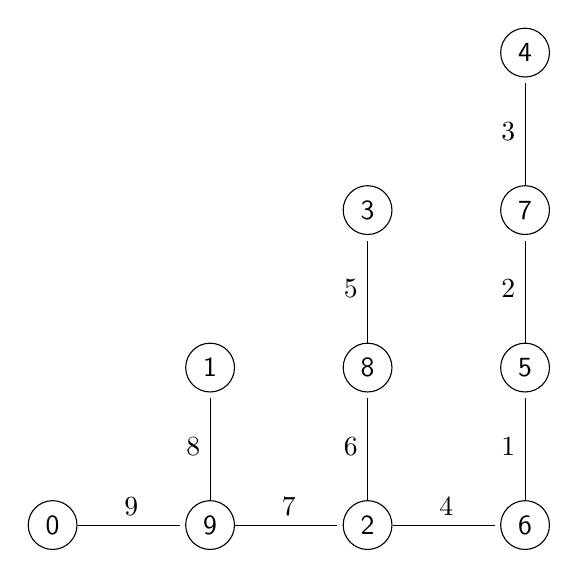
\begin{tikzpicture}[shorten >=2pt, auto, node distance=1cm,
			node_style/.style={circle,draw=black,fill=white!0!,font=\sffamily},
			edge_style/.style={draw=black}]
			
			\node[node_style] (n0) at (0,0)  {0};
			\node[node_style] (n9) at (2,0)  {9};
			\node[node_style] (n2) at (4,0)  {2};
			\node[node_style] (n6) at (6,0)  {6};
			\node[node_style] (n1) at (2,2)  {1};
			\node[node_style] (n8) at (4,2)  {8};
			\node[node_style] (n3) at (4,4)  {3};
			\node[node_style] (n5) at (6,2)  {5};
			\node[node_style] (n7) at (6,4)  {7};
			\node[node_style] (n4) at (6,6)  {4};
			
			
			\draw[edge_style]  (n0) edge node{9} (n9);
			\draw[edge_style]  (n9) edge node{7} (n2);
			\draw[edge_style]  (n2) edge node{4} (n6);
			\draw[edge_style]  (n9) edge node{8} (n1);
			\draw[edge_style]  (n2) edge node{6} (n8);
			\draw[edge_style]  (n8) edge node{5} (n3);
			\draw[edge_style]  (n6) edge node{1} (n5);
			\draw[edge_style]  (n5) edge node{2} (n7);
			\draw[edge_style]  (n7) edge node{3} (n4);
			\end{tikzpicture}}
	\end{center}
	\bigskip

	\item {\bfseries $J_{n,m}$ Trees}\\
	% NEEDS DEFINITION
	A $J_{n,m}$ tree is formed by taking $m$ copies of the $J_n$ tree and making the classification $v_{0,i}=v_{0,j}$ for all $0 {\geq} i$, $j {\geq} m$, provided that $m,n {\geq} 2$. Shown in the figure below is a gracefully-labeled $J_{3,3}$ tree.
	\\
	\begin{center}
		\resizebox {0.5\textwidth} {0.7\height} {
			\begin{tikzpicture}[shorten >=2pt, auto, node distance=1cm,
			node_style/.style={circle,draw=black,fill=white!0!,font=\sffamily},
			edge_style/.style={draw=black}]
			
			\node[node_style] (n0) at (3,0)  {0};
			\node[node_style] (n15) at (5,1)  {15};
			\node[node_style] (n10) at (1,1)  {10};
			\node[node_style] (n5) at (3,-2)  {5};
			\node[node_style] (n12) at (3,-4)  {12};
			\node[node_style] (n11) at (1,-2)  {11};
			\node[node_style] (n4) at (1,-4)  {4};
			\node[node_style] (n13) at (-1,-4)  {5};
			\node[node_style] (n7) at (-1,2)  {7};
			\node[node_style] (n6) at (3,2)  {6};
			\node[node_style] (n1) at (7,0)  {1};
			\node[node_style] (n2) at (7,2)  {2};
			\node[node_style] (n14) at (9,1)  {14};
			\node[node_style] (n3) at (11,0)  {3};
			\node[node_style] (n9) at (1,3)  {9};
			\node[node_style] (n8) at (3,4)  {8};
			
			\draw[edge_style]  (n0) edge node{10} (n10);
			\draw[edge_style]  (n10) edge node{3} (n7);
			\draw[edge_style]  (n7) edge node{2} (n9);
			\draw[edge_style]  (n9) edge node{1} (n8);
			\draw[edge_style]  (n10) edge node{4} (n6);
			\draw[edge_style]  (n0) edge node{15} (n15);
			\draw[edge_style]  (n15) edge node{14} (n1);
			\draw[edge_style]  (n15) edge node{13} (n2);
			\draw[edge_style]  (n2) edge node{12} (n14);
			\draw[edge_style]  (n14) edge node{11} (n3);
			\draw[edge_style]  (n0) edge node{5} (n5);
			\draw[edge_style]  (n5) edge node{6} (n11);
			\draw[edge_style]  (n5) edge node{7} (n12);
			\draw[edge_style]  (n12) edge node{8} (n4);
			\draw[edge_style]  (n13) edge node{9} (n4);
			
			\end{tikzpicture}}
	\end{center}
	
	\bigskip
	\item {\bfseries $J_n$ + $J_{n+1}$ Trees}\\
	% NEEDS DEFINITION
	A  $J_n$ + $J_{n+1}$ tree is formed considering  $J_n$ and $J_{n+1}$ and making the identification $v_{i,n}=v_{i+n,n+1}$ for all $1\leq i\leq n-1$. Shown in the figure below is a gracefully-labeled $J_2$ + $J_3$ tree.
	\\
	\begin{center}
		\resizebox {0.3\textwidth} {0.7\height} {
			\begin{tikzpicture}[shorten >=2pt, auto, node distance=1cm,
			node_style/.style={circle,draw=black,fill=white!0!,font=\sffamily},
			edge_style/.style={draw=black}]
			
			\node[node_style] (n5) at (0,0)  {5};
			\node[node_style] (n2) at (2,0)  {2};
			\node[node_style] (n4) at (4,0)  {4};
			\node[node_style] (n3) at (6,0)  {3};
			\node[node_style] (n6) at (2,2)  {6};
			\node[node_style] (n0) at (2,4)  {0};
			\node[node_style] (n1) at (4,2)  {1};
			
			
			\draw[edge_style]  (n5) edge node{3} (n2);
			\draw[edge_style]  (n2) edge node{2} (n4);
			\draw[edge_style]  (n4) edge node{1} (n3);
			\draw[edge_style]  (n2) edge node{4} (n6);
			\draw[edge_style]  (n0) edge node{6} (n6);
			\draw[edge_style]  (n6) edge node{5} (n1);
			
			
			\end{tikzpicture}}
	\end{center}
	
\end{enumerate}




\section{Objectives}

\noindent This seminar aims:
\begin{itemize}
	\item[a.] to present sufficient background information about the Graceful Tree Conjecture;
	\item[b.] to provide examples of some families of trees that have been shown to be graceful; and 
	\item[c.] to present at least one new family of trees that is not yet shown to be graceful.
\end{itemize}
\section{Results}
This chapter presents a new family of graceful trees. \bigskip
\begin{define}
	For $n\geq2$, let  $F_{n}\left ( 2 \right )$ be the tree formed by \begin{enumerate}
		\item considering a $J_{n}$ tree or a path $v_{0}v_{1}v_{2}\ldots v_{n-1}$ of length $n−1$ and planting to every vertex $v_{i}$ an end vertex of a path of length $i$ for	$i = 0,1,2,\ldots,n−1$ then
		\item planting an end vertex of a path $\overline{P_{2}}$ of length $2$ to every vertex $v_{1}v_{2},\ldots,v_{n}$ of $J_{n}$.
	\end{enumerate}
\end{define}

In the figure below, we illustrate how to construct  $F_{n}\left ( 2 \right )$. 

For $n=2$, $F_{2}\left ( 2 \right )$ is formed by considering a  $J_{2}$ tree and planting an end vertex of a path $\overline{P_{2}}$ of length $2$ to every vertex of $J_{2}$ except $v_{0}$.


\begin{center}
	\resizebox {0.2\textwidth} {0.5\height} {
		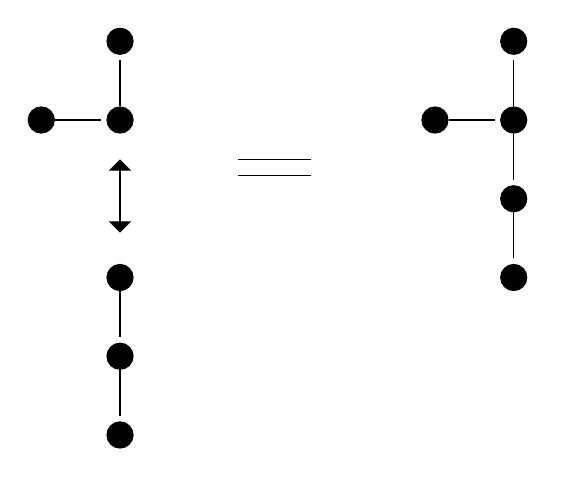
\begin{tikzpicture}[shorten >=2pt, auto, node distance=1cm,
		node_style/.style={circle,draw=black,fill=black,font=\sffamily},
		edge_style/.style={draw=black}]
		
		\node[node_style] (v0) at (1,0)  {};
		\node[node_style] (v1) at (2,0)  {};
		\node[node_style] (a) at (2,1)  {};
		\node[node_style] (f1) at (6,0)  {};
		\node[node_style] (f2) at (7,0)  {};
		\node[node_style] (b) at (7,1)  {};
		\node[node_style] (q1) at (7,-1)  {};
		\node[node_style] (q2) at (7,-2)  {};	
		\node[node_style] (p1) at (2,-2)  {};
		\node[node_style] (p2) at (2,-3)  {};			
		\node[node_style] (p3) at (2,-4)  {};		
		
		\draw[edge_style]  (v0) edge node{} (v1);
		\draw[edge_style]  (v1) edge node{} (a);
		\draw[edge_style]  (p1) edge node{} (p2);
		\draw[edge_style]  (p2) edge node{} (p3);
		\draw[edge_style]  (f1) edge node{} (f2);
		\draw[edge_style]  (f2) edge node{} (b);
		\draw[edge_style]  (f2) edge node{} (q1);
		\draw[edge_style]  (q1) edge node{} (q2);

		\draw[>=triangle 90, <->]
		(2,-0.5) -- (2,-1.5);
		\draw[>=triangle 90, -]
		(3.5,-0.5) -- (4.5,-0.5);
		\draw[>=triangle 90, -]
		(3.5,-0.7) -- (4.5,-0.7);
		
		
		\end{tikzpicture}}
\end{center}

\bigskip

For $n=3$, $F_{3}\left ( 2 \right )$ is formed by considering a  $J_{3}$ tree and planting an end vertex of a path $\overline{P_{2}}$ of length $2$ to every vertex of $J_{3}$ except $v_{0}$.


\begin{center}
	\resizebox {0.2\textwidth} {0.5\height} {
		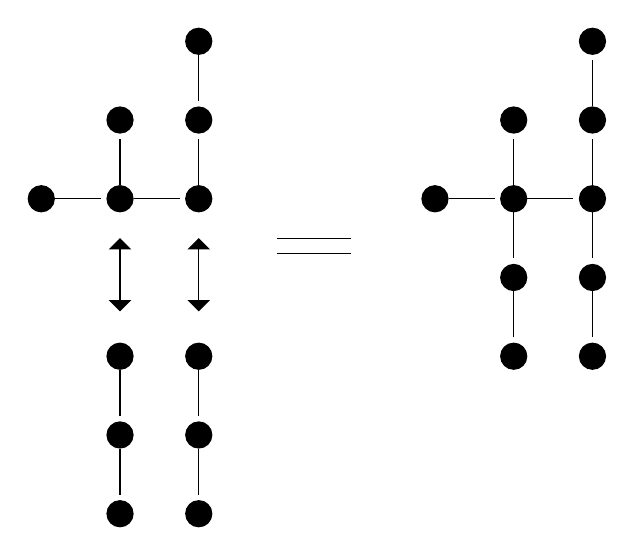
\begin{tikzpicture}[shorten >=2pt, auto, node distance=1cm,
		node_style/.style={circle,draw=black,fill=black,font=\sffamily},
		edge_style/.style={draw=black}]
		
		
		%Jn tree
		\node[node_style] (v0) at (1,0)  {};
		\node[node_style] (v1) at (2,0)  {};
		\node[node_style] (v2) at (3,0) {};
		\node[node_style] (a) at (2,1)  {};
		\node[node_style] (b) at (3,1)  {};
		\node[node_style] (c) at (3,2)  {};		
		\draw[edge_style]  (v0) edge node{} (v1);
		\draw[edge_style]  (v1) edge node{} (a);
		\draw[edge_style]  (v1) edge node{} (v2);
		\draw[edge_style]  (v2) edge node{} (b);
		\draw[edge_style]  (c) edge node{} (b);
		%arrow
		\draw[>=triangle 90, <->]
		(2,-0.5) -- (2,-1.5);
		\draw[>=triangle 90, <->]
		(3,-0.5) -- (3,-1.5);		
	
		%path
		\node[node_style] (p1) at (2,-2)  {};
		\node[node_style] (p2) at (2,-3)  {};			
		\node[node_style] (p3) at (2,-4)  {};
		\node[node_style] (p4) at (3,-2)  {};
		\node[node_style] (p5) at (3,-3)  {};			
		\node[node_style] (p6) at (3,-4)  {};		
		
		\draw[edge_style]  (p1) edge node{} (p2);
		\draw[edge_style]  (p2) edge node{} (p3);
		\draw[edge_style]  (p4) edge node{} (p5);
		\draw[edge_style]  (p5) edge node{} (p6);		
		
		%equal sign
		\draw[>=triangle 90, -]
		(4,-0.5) -- (5,-0.5);
		\draw[>=triangle 90, -]
		(4,-0.7) -- (5,-0.7);
		
		%resulting graph
		\node[node_style] (f1) at (6,0)  {};
		\node[node_style] (f2) at (7,0)  {};
		\node[node_style] (1) at (7,1)  {};
		\node[node_style] (f3) at (8,0) {};
		\node[node_style] (2) at (8,1) {};
		\node[node_style] (3) at (8,2) {};		
		\node[node_style] (q1) at (7,-1)  {};
		\node[node_style] (q2) at (7,-2)  {};
		\node[node_style] (q3) at (8,-1)  {};
		\node[node_style] (q4) at (8,-2)  {};	

		\draw[edge_style]  (f1) edge node{} (f2);
		\draw[edge_style]  (f2) edge node{} (f3);
		\draw[edge_style]  (f2) edge node{} (1);
		\draw[edge_style]  (f3) edge node{} (2);
		\draw[edge_style]  (2) edge node{} (3);
		\draw[edge_style]  (f3) edge node{} (q3);
		\draw[edge_style]  (q3) edge node{} (q4);
		\draw[edge_style]  (f2) edge node{} (q1);
		\draw[edge_style]  (q1) edge node{} (q2);
		
		\end{tikzpicture}}
\end{center}
\bigskip
Note that $n=3$, $F_{3}\left ( 2 \right )$ can also be formed by considering $n=2$, $F_{2}\left ( 2 \right )$ and path $\overline{P_{4}}=p_{0}p_{1}p_{2}p_{3}$ of length $4$ and
joining the vertex $v_{1}$ of  $F_{2}\left ( 2 \right )$ to $p_{2}$ of $\overline{P_{4}}$ by an edge. This property will be important in formulating conjectures for the graceful numbering of any member of the family of trees.

\begin{center}
	\resizebox {0.2\textwidth} {0.5\height} {
		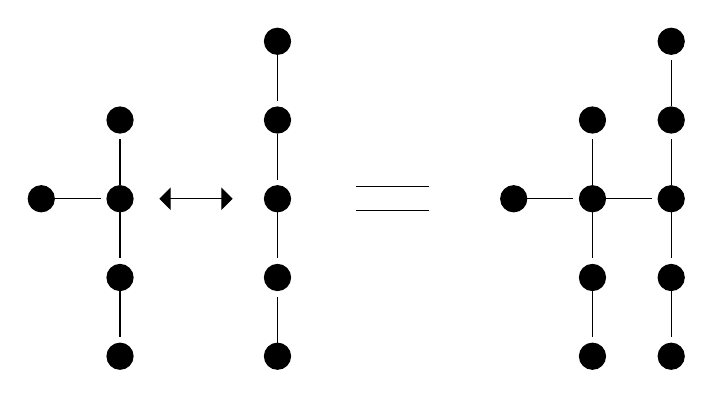
\begin{tikzpicture}[shorten >=2pt, auto, node distance=1cm,
		node_style/.style={circle,draw=black,fill=black,font=\sffamily},
		edge_style/.style={draw=black}]
		
		
		%Jn tree
		\node[node_style] (v0) at (1,0)  {};
		\node[node_style] (v1) at (2,0)  {};
		\node[node_style] (v2) at (2,-1) {};
		\node[node_style] (v3) at (2,-2) {};
		\node[node_style] (a) at (2,1)  {};
	
		\draw[edge_style]  (v0) edge node{} (v1);
		\draw[edge_style]  (v1) edge node{} (a);
		\draw[edge_style]  (v1) edge node{} (v2);
		\draw[edge_style]  (v2) edge node{} (v3);

		%arrow
		\draw[>=triangle 90, <->]
		(2.5,0) -- (3.5,0);

		%path
		\node[node_style] (p1) at (4,2)  {};
		\node[node_style] (p2) at (4,1)  {};			
		\node[node_style] (p3) at (4,0)  {};
		\node[node_style] (p4) at (4,-1)  {};
		\node[node_style] (p5) at (4,-2)  {};			
	
		
		\draw[edge_style]  (p1) edge node{} (p2);
		\draw[edge_style]  (p2) edge node{} (p3);
		\draw[edge_style]  (p3) edge node{} (p4);
		\draw[edge_style]  (p5) edge node{} (p4);		
		
		%equal sign
		\draw[>=triangle 90, -]
		(5,0.15) -- (6,0.15);
		\draw[>=triangle 90, -]
		(5,-0.15) -- (6,-0.15);
		
		%resulting graph
		\node[node_style] (f1) at (7,0)  {};
		\node[node_style] (f2) at (8,0)  {};
		\node[node_style] (1) at (8,1)  {};
		\node[node_style] (f3) at (9,0) {};
		\node[node_style] (2) at (9,1) {};
		\node[node_style] (3) at (9,2) {};		
		\node[node_style] (q1) at (8,-1)  {};
		\node[node_style] (q2) at (8,-2)  {};
		\node[node_style] (q3) at (9,-1)  {};
		\node[node_style] (q4) at (9,-2)  {};	
		
		\draw[edge_style]  (f1) edge node{} (f2);
		\draw[edge_style]  (f2) edge node{} (f3);
		\draw[edge_style]  (f2) edge node{} (1);
		\draw[edge_style]  (f3) edge node{} (2);
		\draw[edge_style]  (2) edge node{} (3);
		\draw[edge_style]  (f3) edge node{} (q3);
		\draw[edge_style]  (q3) edge node{} (q4);
		\draw[edge_style]  (f2) edge node{} (q1);
		\draw[edge_style]  (q1) edge node{} (q2);
		\end{tikzpicture}}
\end{center}

A numbering scheme will now be discussed to gracefully number $F_{n}\left ( 2 \right )$ for $n=2,3,4,5,6$. Given an $F_{n}\left ( 2 \right )$ tree, number the vertices and edges as shown below.

\begin{center}
	\resizebox {0.5\width} {0.5\height} {
		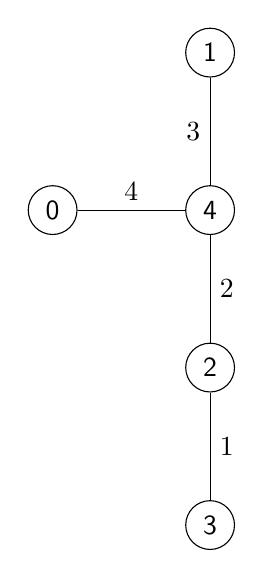
\begin{tikzpicture}[auto, node distance=3cm,
		node_style/.style={circle,draw=black,fill=white!20!,font=\sffamily},
		edge_style/.style={draw=black}]
		
		\node[node_style] (f1) at (6,0)  {0};
		\node[node_style] (f2) at (8,0)  {4};
		\node[node_style] (b) at (8,2)  {1};
		\node[node_style] (q1) at (8,-2)  {2};
		\node[node_style] (q2) at (8,-4)  {3};	
		
		
		\draw[edge_style]  (f1) edge node{4} (f2);
		\draw[edge_style]  (f2) edge node{3} (b);
		\draw[edge_style]  (f2) edge node{2} (q1);
		\draw[edge_style]  (q1) edge node{1} (q2);
		\end{tikzpicture}}\\
		A gracefully-labeled $F_{2}\left ( 2 \right )$ tree
	

	\resizebox {0.5\width} {0.5\height} {
		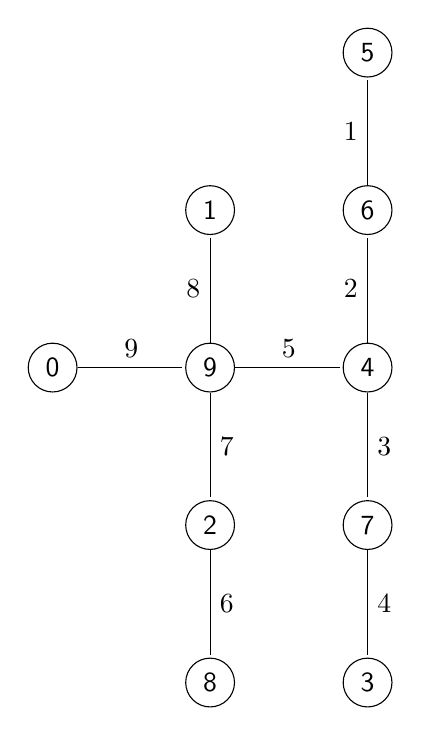
\begin{tikzpicture}[shorten >=1pt, auto, node distance=5cm,
		node_style/.style={circle,draw=black,fill=white!20!,font=\sffamily},
		edge_style/.style={draw=black}]
		
		%resulting graph
		\node[node_style] (f1) at (0,0)  {0};
		\node[node_style] (f2) at (2,0)  {9};
		\node[node_style] (1) at (2,2)  {1};
		\node[node_style] (f3) at (4,0) {4};
		\node[node_style] (2) at (4,2) {6};
		\node[node_style] (3) at (4,4) {5};		
		\node[node_style] (q1) at (2,-2)  {2};
		\node[node_style] (q2) at (2,-4)  {8};
		\node[node_style] (q3) at (4,-2)  {7};
		\node[node_style] (q4) at (4,-4)  {3};	
		
		\draw[edge_style]  (f1) edge node{9} (f2);
		\draw[edge_style]  (f2) edge node{5} (f3);
		\draw[edge_style]  (f2) edge node{8} (1);
		\draw[edge_style]  (f3) edge node{2} (2);
		\draw[edge_style]  (2) edge node{1} (3);
		\draw[edge_style]  (f3) edge node{3} (q3);
		\draw[edge_style]  (q3) edge node{4} (q4);
		\draw[edge_style]  (f2) edge node{7} (q1);
		\draw[edge_style]  (q1) edge node{6} (q2);
		\end{tikzpicture}}
	
		A gracefully-labeled $F_{3}\left ( 2 \right )$ tree
	
\end{center}
	
	


\begin{center}
	\resizebox {0.5\width} {0.5\height} {
		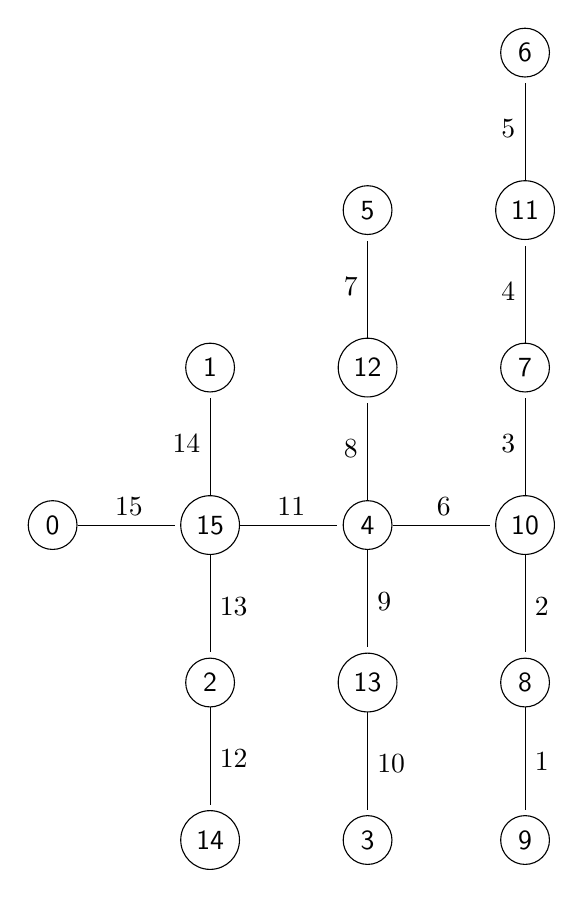
\begin{tikzpicture}[shorten >=2pt, auto, node distance=1cm,
		node_style/.style={circle,draw=black,fill=white!20!,font=\sffamily},
		edge_style/.style={draw=black}]
		
		%resulting graph
		\node[node_style] (f1) at (0,0)  {0};
		\node[node_style] (f2) at (2,0)  {15};
		\node[node_style] (f3) at (4,0) {4};
		\node[node_style] (f4) at (6,0)  {10};
		\node[node_style] (1) at (2,2)  {1};
		\node[node_style] (2) at (4,2) {12};
		\node[node_style] (3) at (4,4) {5};	
		\node[node_style] (4) at (6,2) {7};		
		\node[node_style] (5) at (6,4) {11};		
		\node[node_style] (6) at (6,6) {6};	
		\node[node_style] (q1) at (2,-2)  {2};
		\node[node_style] (q2) at (2,-4)  {14};
		\node[node_style] (q3) at (4,-2)  {13};
		\node[node_style] (q4) at (4,-4)  {3};
		\node[node_style] (q5) at (6,-2)  {8};
		\node[node_style] (q6) at (6,-4)  {9};	
		
		\draw[edge_style]  (f1) edge node{15} (f2);
		\draw[edge_style]  (f2) edge node{11} (f3);
		\draw[edge_style]  (f3) edge node{6} (f4);
		\draw[edge_style]  (f2) edge node{14} (1);
		\draw[edge_style]  (f3) edge node{8} (2);
		\draw[edge_style]  (2) edge node{7} (3);
		\draw[edge_style]  (f4) edge node{3} (4);
		\draw[edge_style]  (4) edge node{4} (5);
		\draw[edge_style]  (5) edge node{5} (6);
		\draw[edge_style]  (f3) edge node{9} (q3);
		\draw[edge_style]  (q3) edge node{10} (q4);
		\draw[edge_style]  (f2) edge node{13} (q1);
		\draw[edge_style]  (q1) edge node{12} (q2);
		\draw[edge_style]  (f4) edge node{2} (q5);
		\draw[edge_style]  (q5) edge node{1} (q6);
		\end{tikzpicture}}
	\begin{center}
		A gracefully-labeled $F_{4}\left ( 2 \right )$ tree
	\end{center}
\end{center}

\begin{center}
	\resizebox {0.5\width} {0.5\height} {
		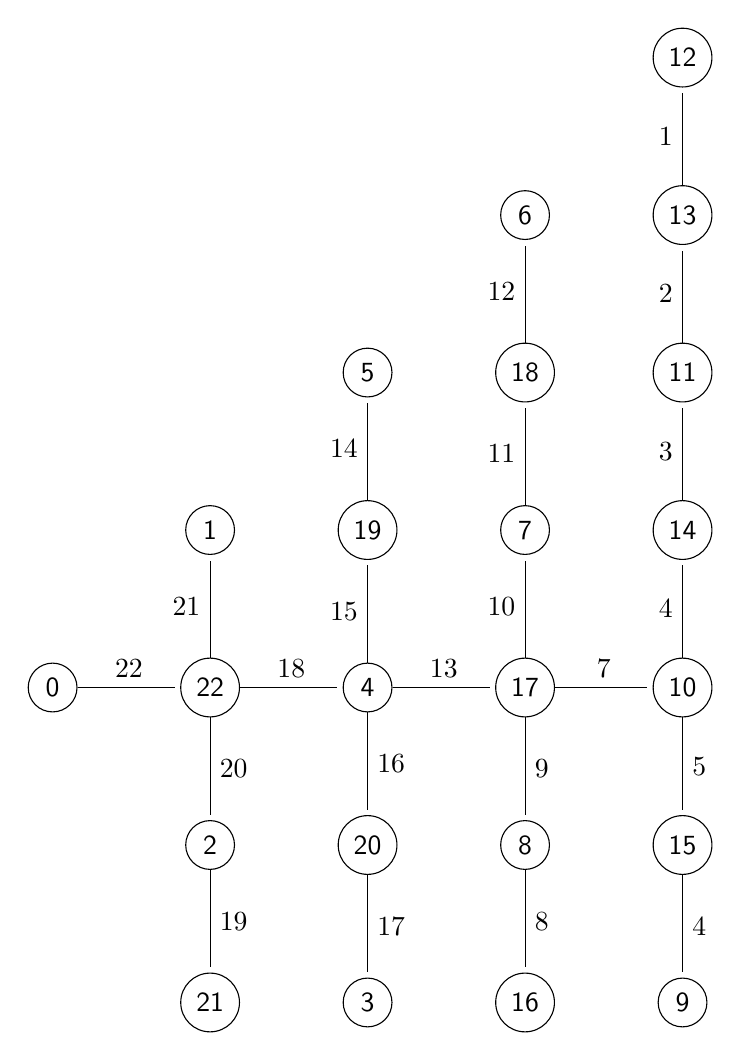
\begin{tikzpicture}[shorten >=2pt, auto, node distance=1cm,
		node_style/.style={circle,draw=black,fill=white!20!,font=\sffamily},
		edge_style/.style={draw=black}]
		
		%resulting graph
		\node[node_style] (f1) at (0,0)  {0};
		\node[node_style] (f2) at (2,0)  {22};
		\node[node_style] (f3) at (4,0) {4};
		\node[node_style] (f4) at (6,0)  {17};
		\node[node_style] (f5) at (8,0)  {10};
		\node[node_style] (1) at (2,2)  {1};
		\node[node_style] (2) at (4,2) {19};
		\node[node_style] (3) at (4,4) {5};	
		\node[node_style] (4) at (6,2) {7};		
		\node[node_style] (5) at (6,4) {18};		
		\node[node_style] (6) at (6,6) {6};
		\node[node_style] (7) at (8,2)  {14};
		\node[node_style] (8) at (8,4)  {11};
		\node[node_style] (9) at (8,6)  {13};
		\node[node_style] (10) at (8,8)  {12};	
		\node[node_style] (q1) at (2,-2)  {2};
		\node[node_style] (q2) at (2,-4)  {21};
		\node[node_style] (q3) at (4,-2)  {20};
		\node[node_style] (q4) at (4,-4)  {3};
		\node[node_style] (q5) at (6,-2)  {8};
		\node[node_style] (q6) at (6,-4)  {16};	
		\node[node_style] (q7) at (8,-2)  {15};
		\node[node_style] (q8) at (8,-4)  {9};
		
		\draw[edge_style]  (f1) edge node{22} (f2);
		\draw[edge_style]  (f2) edge node{18} (f3);
		\draw[edge_style]  (f3) edge node{13} (f4);
		\draw[edge_style]  (f4) edge node{7} (f5);
		\draw[edge_style]  (f5) edge node{4} (7);
		\draw[edge_style]  (7) edge node{3} (8);
		\draw[edge_style]  (8) edge node{2} (9);
		\draw[edge_style]  (9) edge node{1} (10);
		\draw[edge_style]  (f2) edge node{21} (1);
		\draw[edge_style]  (f3) edge node{15} (2);
		\draw[edge_style]  (2) edge node{14} (3);
		\draw[edge_style]  (f4) edge node{10} (4);
		\draw[edge_style]  (4) edge node{11} (5);
		\draw[edge_style]  (5) edge node{12} (6);
		\draw[edge_style]  (f3) edge node{16} (q3);
		\draw[edge_style]  (q3) edge node{17} (q4);
		\draw[edge_style]  (f2) edge node{20} (q1);
		\draw[edge_style]  (q1) edge node{19} (q2);
		\draw[edge_style]  (f4) edge node{9} (q5);
		\draw[edge_style]  (q5) edge node{8} (q6);
		\draw[edge_style]  (f5) edge node{5} (q7);
		\draw[edge_style]  (q7) edge node{4} (q8);
		\end{tikzpicture}}
	\begin{center}
		A gracefully-labeled $F_{5}\left ( 2 \right )$ tree
	\end{center}



	\resizebox {0.5\width} {0.5\height} {
		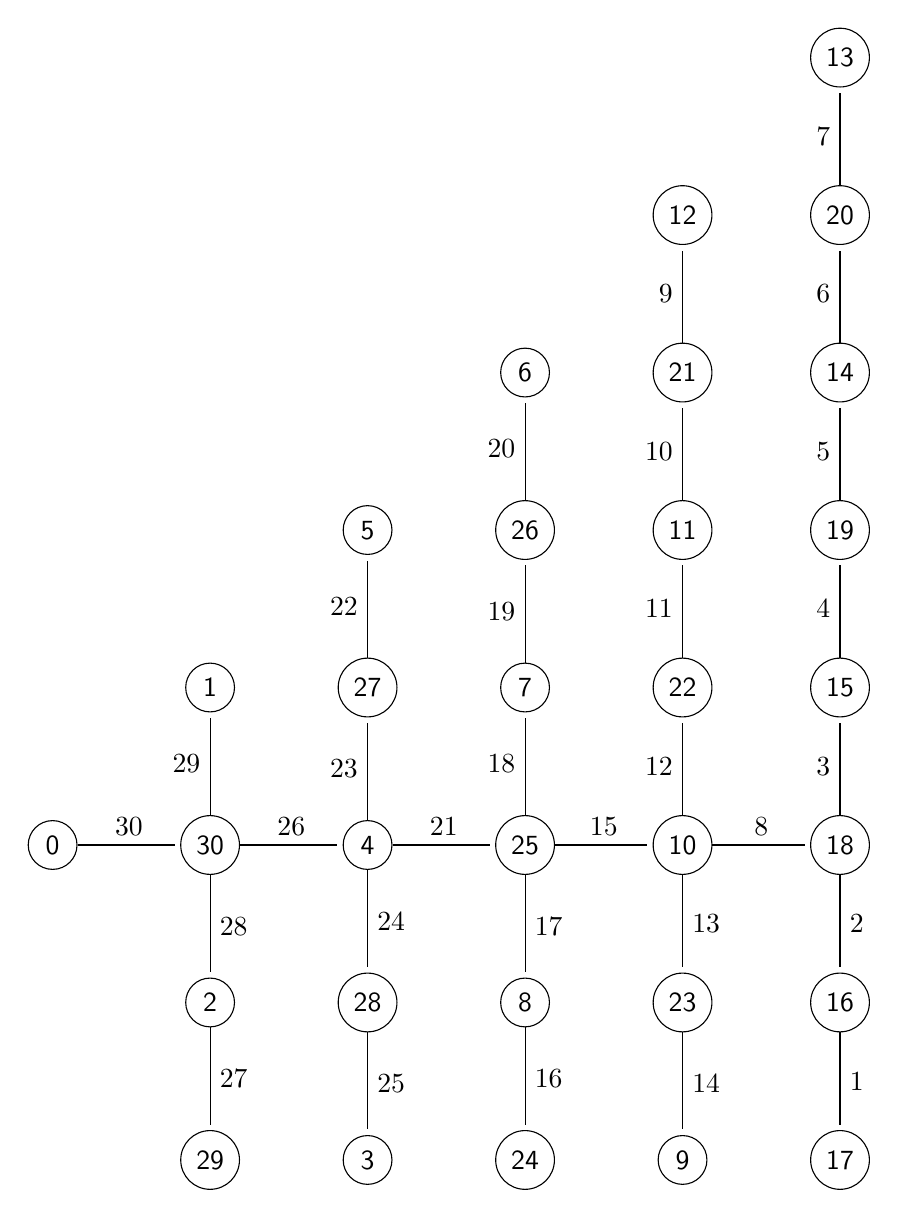
\begin{tikzpicture}[shorten >=2pt, auto, node distance=1cm,
		node_style/.style={circle,draw=black,fill=white!20!,font=\sffamily},
		edge_style/.style={draw=black}]
		
		%resulting graph
		\node[node_style] (f1) at (0,0)  {0};
		\node[node_style] (f2) at (2,0)  {30};
		\node[node_style] (f3) at (4,0) {4};
		\node[node_style] (f4) at (6,0)  {25};
		\node[node_style] (f5) at (8,0)  {10};
		\node[node_style] (f6) at (10,0)  {18};
		\node[node_style] (1) at (2,2)  {1};
		\node[node_style] (2) at (4,2) {27};
		\node[node_style] (3) at (4,4) {5};	
		\node[node_style] (4) at (6,2) {7};		
		\node[node_style] (5) at (6,4) {26};		
		\node[node_style] (6) at (6,6) {6};
		\node[node_style] (7) at (8,2)  {22};
		\node[node_style] (8) at (8,4)  {11};
		\node[node_style] (9) at (8,6)  {21};
		\node[node_style] (10) at (8,8)  {12};
		\node[node_style] (11) at (10,2)  {15};
		\node[node_style] (12) at (10,4)  {19};
		\node[node_style] (13) at (10,6)  {14};
		\node[node_style] (14) at (10,8)  {20};
		\node[node_style] (15) at (10,10)  {13};	
		\node[node_style] (q1) at (2,-2)  {2};
		\node[node_style] (q2) at (2,-4)  {29};
		\node[node_style] (q3) at (4,-2)  {28};
		\node[node_style] (q4) at (4,-4)  {3};
		\node[node_style] (q5) at (6,-2)  {8};
		\node[node_style] (q6) at (6,-4)  {24};	
		\node[node_style] (q7) at (8,-2)  {23};
		\node[node_style] (q8) at (8,-4)  {9};
		\node[node_style] (q9) at (10,-2)  {16};
		\node[node_style] (q10) at (10,-4)  {17};
		
		\draw[edge_style]  (f1) edge node{30} (f2);
		\draw[edge_style]  (f2) edge node{26} (f3);
		\draw[edge_style]  (f3) edge node{21} (f4);
		\draw[edge_style]  (f4) edge node{15} (f5);
		\draw[edge_style]  (f5) edge node{8} (f6);
		\draw[edge_style]  (f6) edge node{3} (11);
		\draw[edge_style]  (11) edge node{4} (12);
		\draw[edge_style]  (12) edge node{5} (13);
		\draw[edge_style]  (13) edge node{6} (14);
		\draw[edge_style]  (14) edge node{7} (15);
		\draw[edge_style]  (f5) edge node{12} (7);
		\draw[edge_style]  (7) edge node{11} (8);
		\draw[edge_style]  (8) edge node{10} (9);
		\draw[edge_style]  (9) edge node{9} (10);
		\draw[edge_style]  (f2) edge node{29} (1);
		\draw[edge_style]  (f3) edge node{23} (2);
		\draw[edge_style]  (2) edge node{22} (3);
		\draw[edge_style]  (f4) edge node{18} (4);
		\draw[edge_style]  (4) edge node{19} (5);
		\draw[edge_style]  (5) edge node{20} (6);
		\draw[edge_style]  (f3) edge node{24} (q3);
		\draw[edge_style]  (q3) edge node{25} (q4);
		\draw[edge_style]  (f2) edge node{28} (q1);
		\draw[edge_style]  (q1) edge node{27} (q2);
		\draw[edge_style]  (f4) edge node{17} (q5);
		\draw[edge_style]  (q5) edge node{16} (q6);
		\draw[edge_style]  (f5) edge node{13} (q7);
		\draw[edge_style]  (q7) edge node{14} (q8);
		\draw[edge_style]  (f6) edge node{2} (q9);
		\draw[edge_style]  (q9) edge node{1} (q10);
		\end{tikzpicture}}

		A gracefully-labeled $F_{6}\left ( 2 \right )$ tree

\end{center}
\section{Conclusion}

In this study, we were able to present sufficient background information about the Graceful Tree Conjecture. Moreover, we were able to provide examples of some families of trees that have been shown to be graceful. Finally, we have shown that and for $n\geq2$, if we consider a $J_{n}$ tree or a path $v_{0}v_{1}v_{2}\ldots v_{n-1}$ of length $n−1$ and planting to every vertex $v_{i}$ an end vertex of a path of length $i$ for
$i = 0,1,2,\ldots,n−1$ then if we plant an end vertex of a path $\overline{P_{2}}$ of length $2$ to every vertex $v_{1}v_{2},\ldots,v_{n}$ of $J_{n}$, we will come up with $J_{n}$ which is shown to have a graceful-labeling. 

The discovery and development of another class or family of graceful treeas further strengthens the Graceful Tree Conjecture which is yet to be proven.


\section{References}
\begin{itemize}
	\item Eshigo, Kourosh (2002, September). Introduction to Graceful Graphs. Sharif University of Technology
	\item Horton, Michael P. (2003, November). Greaceful trees: statistiics and algorithms. University of Tasmania.
	\item Morgan, David (2008), ”All lobsters with perfect matchings are graceful”, Bulletin of the Institute of Combinatorics and its Applications, 53: 8285.
	\item Watson, Lynn (2000). A Survey on Graceful Labeling of Graphs. University of Colorado at Denver.
\end{itemize}


\end{document}